\documentclass[tikz,border=0pt]{standalone}
\pdfminorversion=7
\usepackage[T1]{fontenc}
\usepackage{lmodern,amsmath,amssymb,graphicx}
\usepackage{pgfplots}
\usetikzlibrary{arrows.meta,calc,positioning,patterns,decorations.pathreplacing}
\pgfplotsset{compat=1.18}
\definecolor{family}{RGB}{0,140,18}
\definecolor{familypale}{RGB}{225,255,226}
\definecolor{frozen}{RGB}{49,57,208}
\definecolor{frozenpale}{RGB}{234,235,255}
\definecolor{adapter}{RGB}{219,102,0}
\definecolor{adapterpale}{RGB}{255,196,135}
\definecolor{outputcol}{RGB}{120,38,130}
\definecolor{ink}{RGB}{33,33,33}
\definecolor{muted}{RGB}{105,105,105}
\tikzset{
 figure/.style={x=1pt,y=1pt,line cap=round,line join=round,text=ink,
   >={Stealth[length=7pt,width=6pt]},font=\fontsize{20}{24}\selectfont},
 title/.style={font=\fontsize{29}{33}\selectfont},
 heading/.style={font=\fontsize{22}{26}\selectfont},
 labeltext/.style={font=\fontsize{18}{22}\selectfont,align=center},
 smalllabel/.style={font=\fontsize{15}{19}\selectfont,align=center},
 equation/.style={font=\fontsize{24}{29}\selectfont,align=center},
 flow/.style={->,line width=1.3pt},
 fineflow/.style={->,line width=.8pt},
 target/.style={circle,fill=family,draw=white,line width=1.2pt,inner sep=0pt,minimum size=12pt},
 candidate/.style={circle,fill=white,draw=muted,line width=1.3pt,inner sep=0pt,minimum size=10pt},
 neuron/.style={circle,draw=frozen,fill=frozen!18,minimum size=13pt,inner sep=0pt,line width=.8pt}
}
\DeclareMathOperator{\rank}{rank}
\DeclareMathOperator{\row}{row}
\DeclareMathOperator{\col}{col}
\newcommand{\R}{\mathbb R}
\graphicspath{{assets/}}
\newcommand{\canvas}[1]{\path[use as bounding box] (0,0) rectangle (960,600);
  \node[title,anchor=west] at (36,557) {#1};}
\newcommand{\glyphgrid}[2]{
 \begin{scope}[shift={(#1,#2)}]
  \fill[white] (0,0) rectangle (136,136);
  \foreach \x/\y/\c in {1/1/80,2/2/80,2/3/45,3/4/45,3/5/45,4/5/100,4/6/45,5/6/45,5/4/45,5/2/100,6/1/80}{
    \fill[frozen!\c] (\x*17,\y*17) rectangle ++(17,17);
  }
  \draw[step=17pt,black!30,line width=.35pt] (0,0) grid (136,136);
  \draw[black!45,line width=.6pt] (0,0) rectangle (136,136);
 \end{scope}}

\begin{document}
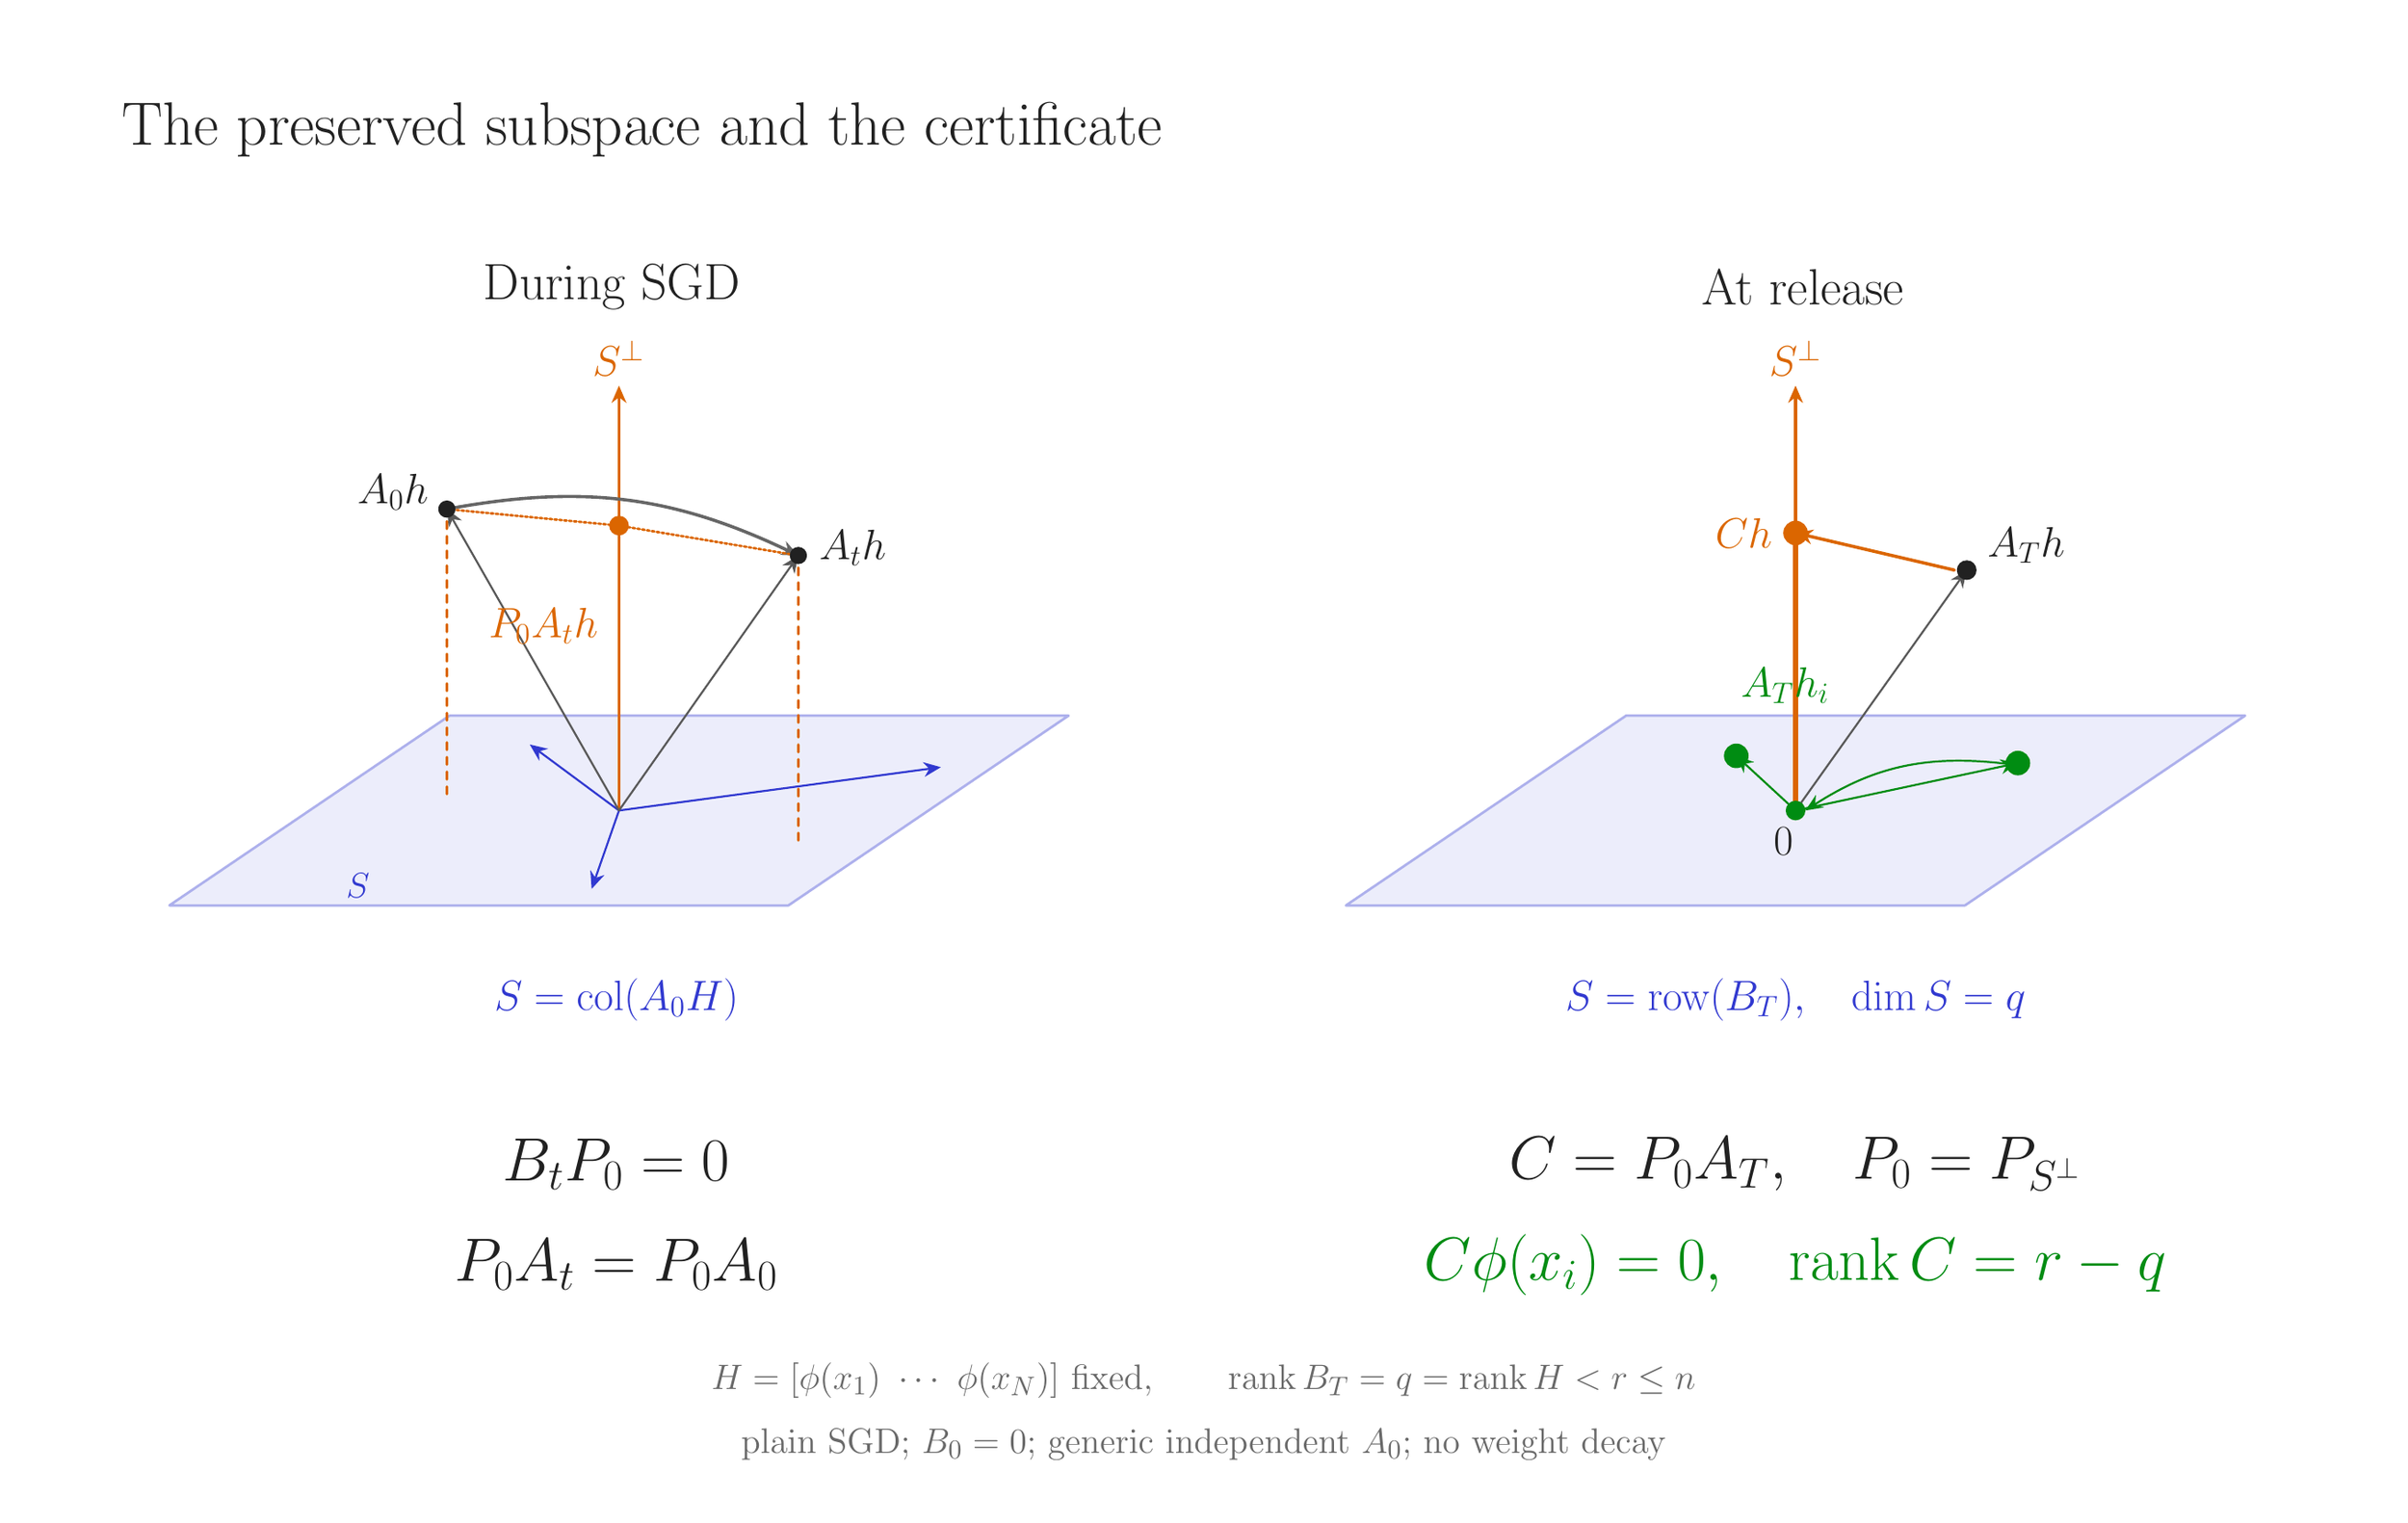
\begin{tikzpicture}[figure]
\canvas{The preserved subspace and the certificate}
\node[heading] at (239,493) {During SGD};
\node[heading] at (724,493) {At release};
\begin{scope}[shift={(242,280)},x={(1pt,0pt)},y={(.62pt,.42pt)},z={(0pt,1pt)}]
 \filldraw[fill=frozen!9,draw=frozen!40,line width=1pt]
  (-126,-92,0)--(126,-92,0)--(126,92,0)--(-126,92,0)--cycle;
 \draw[flow,adapter] (0,0,0)--(0,0,173) node[above,labeltext] {$S^\perp$};
 \draw[fineflow,frozen] (0,0,0)--(105,42,0);
 \draw[fineflow,frozen] (0,0,0)--(-76,64,0);
 \draw[fineflow,frozen] (0,0,0)--(36,-76,0);
 \node[smalllabel,text=frozen] at (-61,-73,0) {$S$};
 \draw[dashed,adapter,line width=1.1pt] (-80,16,0)--(-80,16,116);
 \draw[dashed,adapter,line width=1.1pt] (91,-29,0)--(91,-29,116);
 \draw[fineflow,black!65] (0,0,0)--(-80,16,116);
 \draw[fineflow,black!65] (0,0,0)--(91,-29,116);
 \draw[flow,black!60] (-80,16,116) to[bend left=18] (91,-29,116);
 \draw[densely dotted,adapter,line width=1pt] (-80,16,116)--(0,0,116)--(91,-29,116);
 \fill[adapter] (0,0,116) circle (4pt);
 \fill[ink] (-80,16,116) circle (3.5pt);
 \fill[ink] (91,-29,116) circle (3.5pt);
 \node[labeltext,anchor=east] at (-84,16,123) {$A_0h$};
 \node[labeltext,anchor=west] at (96,-29,119) {$A_th$};
 \node[labeltext,text=adapter,anchor=east] at (-5,0,75) {$P_0A_th$};
\end{scope}
\node[labeltext,text=frozen] at (241,203) {$S=\col(A_0H)$};
\node[equation] at (241,136) {$B_tP_0=0$};
\node[equation] at (241,95) {$P_0A_t=P_0A_0$};
\begin{scope}[shift={(721,280)},x={(1pt,0pt)},y={(.62pt,.42pt)},z={(0pt,1pt)}]
 \filldraw[fill=frozen!9,draw=frozen!40,line width=1pt]
  (-126,-92,0)--(126,-92,0)--(126,92,0)--(-126,92,0)--cycle;
 \draw[flow,adapter] (0,0,0)--(0,0,173) node[above,labeltext] {$S^\perp$};
 \draw[fineflow,draw=family] (0,0,0)--(-57,53,0);
 \draw[fineflow,draw=family] (0,0,0)--(62,46,0);
 \fill[fill=family] (-57,53,0) circle (5pt);
 \fill[fill=family] (62,46,0) circle (5pt);
 \draw[fineflow,black!65] (0,0,0)--(92,-36,113);
 \fill[ink] (92,-36,113) circle (4pt);
 \draw[flow,adapter] (87,-36,113)--(0,0,113);
 \draw[line width=2.5pt,adapter] (0,0,0)--(0,0,113);
 \fill[adapter] (0,0,113) circle (5pt);
 \node[labeltext,anchor=west] at (97,-36,123) {$A_Th$};
 \node[labeltext,text=adapter,anchor=east] at (-6,0,113) {$Ch$};
 \node[labeltext,text=family] at (-47,69,22) {$A_Th_i$};
 \draw[fineflow,draw=family] (59,45,0) to[bend right=20] (4,0,0);
 \fill[fill=family] (0,0,0) circle (4pt);
 \node[labeltext,anchor=north] at (0,-8,0) {$0$};
\end{scope}
\node[labeltext,text=frozen] at (721,203) {$S=\row(B_T),\quad \dim S=q$};
\node[equation] at (721,136) {$C=P_0A_T,\quad P_0=P_{S^\perp}$};
\node[equation,text=family] at (721,95) {$C\phi(x_i)=0,\quad\rank C=r-q$};
\node[smalllabel,text=muted] at (480,48) {$H=[\phi(x_1)\ \cdots\ \phi(x_N)]\ \text{fixed},\qquad
 \rank B_T=q=\rank H<r\le n$};
\node[smalllabel,text=muted] at (480,22) {plain SGD; $B_0=0$; generic independent $A_0$; no weight decay};
\end{tikzpicture}
\end{document}
